\documentclass[11pt, oneside]{article} 
\usepackage{geometry}
\geometry{letterpaper} 
\usepackage{graphicx}
	
\usepackage{amssymb}
\usepackage{amsmath}
\usepackage{parskip}
\usepackage{color}
\usepackage{hyperref}

\graphicspath{{/Users/telliott_admin/Tex/png/}}
% \begin{center} 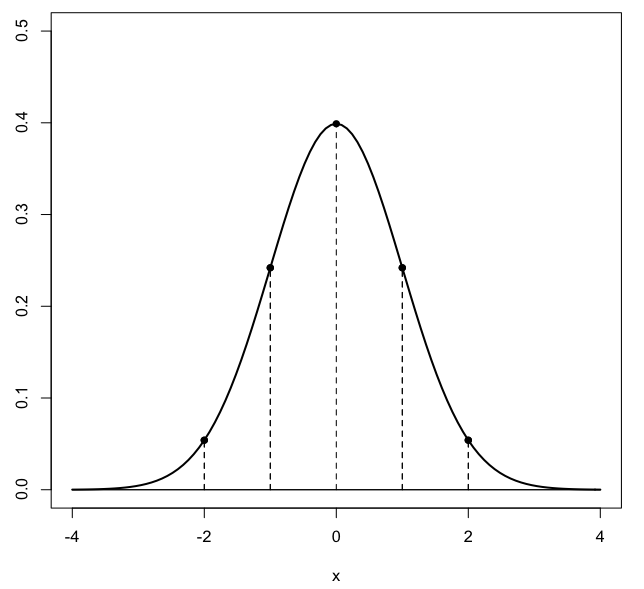
\includegraphics [scale=0.4] {gauss3.png} \end{center}

%break
\title{Parabola geometry}
\date{}

\begin{document}
\maketitle
\Large
\label{sec:Parabola_geometry}
You probably know that the \emph{conic sections} are the parabola, circle and ellipse, and hyperbola.
\begin{center} 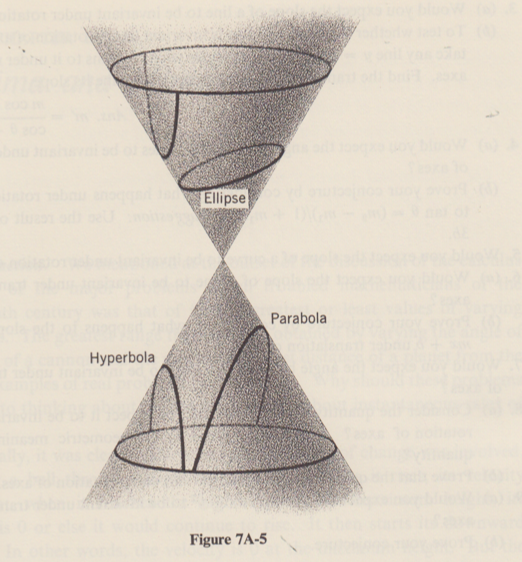
\includegraphics [scale=0.4] {Kline_7A_5.png} \end{center}

After the circle, perhaps the most familiar of these is the parabola.  Consider a parabola in standard orientation, opening up and with its axis of symmetry pointed straight up and down.
\begin{center} 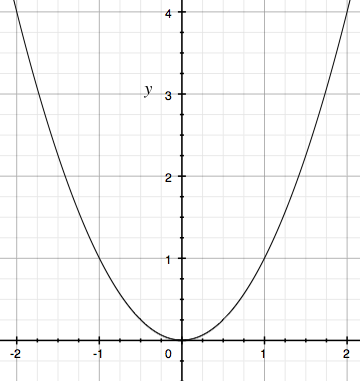
\includegraphics [scale=0.4] {para1.png} \end{center}

A parabola of this orientation whose vertex is located at the origin and with axis of symmetry $x=0$ is described by the very simple equation
\[ y = ax^2 \]
For the one shown above, $a$ is equal to $1$, giving $y = x^2$.  For example, the points $(1,1)$ and $(2,4)$ lie on the curve.

Every parabola contains a term with $x^2$.  If there isn't a power of $x^2$, the curve isn't a parabola.  Notice that $x^2 \ge 0$; hence the minimum value of $y$ is $0$, and the corresponding $x$ is also $0$, and thus the vertex, the point at which the value of $y$ is a minimum, is at $(0,0)$.

Three operations transform the basic parabola $y=x^2$ into any other parabola. 

First, we can multiply by such a constant, usually designated $a$, called the "shape parameter".  You can think of $a$ as a factor that stretches the plane in the y-dimension.  If we re-scale $y$ by substituting $u = y/a$, then $y = ax^2$ becomes $u = x^2$.  Multiplying every $y$ value by $1/a$, without changing $x$, gives the $u$ version.

The parabola can also be moved, or translated, from the origin to a non-centered position with its vertex at $P = (h,k)$.

We can also rotate the parabola, for example so that its axis of symmetry lies along a diagonal like the line $y = x$.  We will look at this in another chapter.

Back to translation.  You've certainly seen this standard equation before
\[ y = ax^2 + bx + c \]
This equation describes a parabola with the vertex at a point other than the origin.  If $b=0$, the axis of symmetry isn't changed, we just add a constant $c$ to each value of $ax^2$ to give the final $y$.  The curve is moved straight up the page ($c > 0$) or down it.

If two parabolas have the same shape but differ only by translation, the $a$ terms must be the same.  The difference---the extra terms
\[ bx + c \]
describe the movement (with a bit of $a$ mixed in).

\subsection*{vertex}
A general way of calculating the $x$ coordinate of the vertex, when it's not at $x=0$, is to use the equation
\[ x = -\frac{b}{2a} \]
where, as before, $b$ refers to $y = ax^2 + bx + c$.  In the case of $y = ax^2$:
\[ x = -\frac{0}{2} = 0 \]

The equation $x = -b/2a$ can be derived from calculus but also by algebraic manipulation.

Suppose the vertex of the parabola $y=x^2$ is at $P=(2,1)$.  
\begin{center} 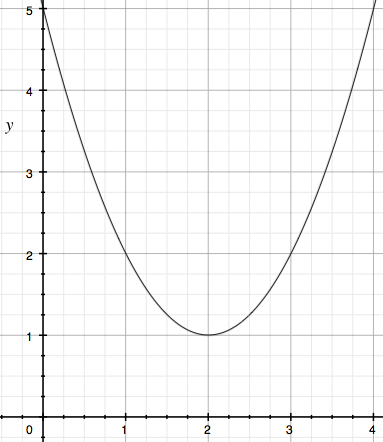
\includegraphics [scale=0.4] {para1b.png} \end{center}

The letters $h$ and $k$ are traditionally used for these values, which are constants for any particular parabola.  For example, here $h=2$ and $k=1$, given the vertex at $(2,1)$.

We write the equation of this parabola as
\[ (y-k) = a(x-h)^2 \]

It may seem counterintuitive that the equation has minus signs (namely, $y-k$ \emph{and} $x-h$), even though the vertex is at $(h,k)$.

One way to see this is to put the $k$ on the other side
\[ y = (x-h)^2 + k \]
Now it's clear that for positive $k$, every $y$ is shifted \emph{up} by $k$ units yet the standard equation contains $y-k$ on the left-hand side.

If we multiply this out (using $a$ to be completely general) we obtain
\[ y = a(x-h)^2 + k \]
\[ y = ax^2 - 2axh + ah^2 + k \]

So, comparing the two forms 
\[ y = ax^2 + bx + c \]
\[ y = ax^2 - 2axh + ah^2 + k \]
We see that the coefficient of the $x$ term is $-2ah$, with
\[ b = -2ah \]
\[ h = -\frac{b}{2a} \]

This is the equation we used above in finding the vertex.  If we know $a$ and $b$ we can calculate $h$, obtaining the $x$-value at the vertex.  Furthermore, from the above result
\[  c = ah^2 + k \]
\[ k = c - ah^2 = c - \frac{b^2}{4a} \]
or alternatively, you can get the same result by just plugging $x=h=-b/2a$ into the original equation.

When we're given an equation in the form $y = ax^2 + bx + c$ and asked to find the vertex $(h,k)$, this is how it's done.

Since the shape factor $a$ is independent of $h$ and $k$, most problems with parabolas can be considered using the version placing its vertex at the origin, without loss of generality.
\subsection*{roots}
The roots of the equation are the points where $y = 0$ so that
\[ y = 0 = ax^2 + bx + c \]
You can solve this either by factoring (in favorable cases) or by using the quadratic formula.

\[ x = \frac{-b \pm \sqrt{b^2 - 4ac}}{2a} \] 
Also, I'm sure you know that if the parabola just touches the x-axis then the discriminant 
\[ D = b^2 - 4ac = 0 \]
whereas if the parabola does not cross the x-axis then $D<0$ and there are no (real) roots.  Just adding a large enough $c$ shifts the parabola up so it doesn't cross the $x$-axis any more.

\hypertarget{completing_the_square}{}
\subsection*{completing the square}

Let's derive the quadratic equation by "completing the square."  First rearrange
\[ y = ax^2 + bx + c \]
\[ \frac{(y-c)}{a} = x^2 + \frac{bx}{a} \]
The crucial step is to observe that if we add the correct amount to the right-hand side, it can be factored as a perfect square.

\[ x^2 + \frac{bx}{a} + (\frac{b}{2a})^2 \]
\[ = (x + \frac{b}{2a})(x + \frac{b}{2a}) \]
\[ = (x + \frac{b}{2a})^2 \]
Of course, to maintain the equality we must add the same term to the left-hand side

\[ \frac{y-c}{a} + (\frac{b}{2a})^2 \]
\[ \frac{1}{a} \ [ \ y - c + \frac{b^2}{4a} \ ] \]
Combining the two results
\[ \frac{1}{a} \ [ \ y - c + \frac{b^2}{4a} \ ] \ = (x + \frac{b}{2a})^2 \] 
\[ y-c + \frac{b^2}{4a} = a(x + \frac{b}{2a})^2 \]

You may recognize $h$ and $k$ in this completed square (or rather $-h$ and $-k$), but if not, take a moment to go back and compare with the equations we had before.  

Now, the roots are just the points when $y=0$ and so
\[  -c + \frac{b^2}{4a} = a(x + \frac{b}{2a})^2 \]
\[  \frac{b^2 -4ac}{4a} = a(x + \frac{b}{2a})^2 \]
\[  \frac{b^2-4ac}{4a^2} = (x + \frac{b}{2a})^2 \]
\[  x + \frac{b}{2a} = \pm \frac{\sqrt{b^2-4ac}}{2a}  \]
\[  x = \frac{-b \pm \sqrt{b^2-4ac}}{2a} \]
which is the quadratic equation.

Most sources credit Brahmagupta with this idea.
\begin{quote}To the absolute number multiplied by four times the [coefficient of the] square, add the square of the [coefficient of the] middle term; the square root of the same, less the [coefficient of the] middle term, being divided by twice the [coefficient of the] square is the value.\end{quote}

Occasionally you will see credit given to al-Khwarizmi, but the general opinion is that he transcribed the Indian sources.

\subsection*{slope}
Using calculus, for a parabola in standard orientation, we can find the slope of the tangent line to the curve at any point by taking the derivative
\[ m = \frac{d}{dx} (ax^2 + bx + c) = 2ax + b \]

The slope of the tangent is zero at the vertex
\[ m = 2ax + b = 0 \]
\[ x = -\frac{b}{2a} \]
as we saw before.

\subsection*{Headlight problem}

One of the most interesting properties of the parabola is that any light ray coming down vertically will bounce off the surface of the parabola so that it is reflected to the focus.  Reflecting telescopes are made in this way.  The reverse is also true.  The inside of a headlight has a parabolic shape, so that the light emitted from a bulb at the focus, bounces off the inside surface to form a parallel beam.

\subsection*{parallel rays are reflected to the focus}
Above we said that if the light source is placed at the focus of a paraboloid headlight, then rays reflected off the surface emerge "straight out" (or up, as we usually draw parabolas).  Conversely, light rays parallel to the axis of symmetry that enter a paraboloid converge at the focus.

\begin{center} 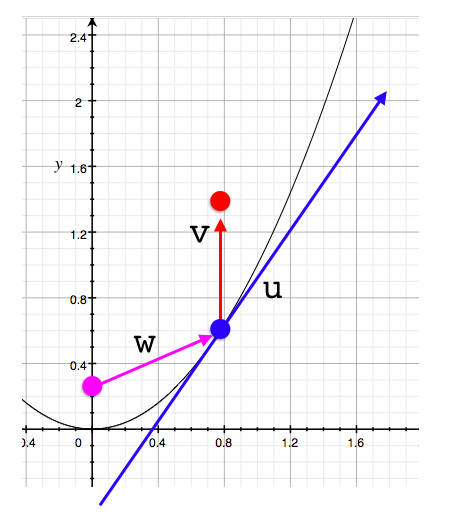
\includegraphics [scale=0.5] {headlight.png} \end{center}

We will prove this here using vectors, making use of the property from optics that a reflected ray makes equal angles of incidence and reflection.

We pick an arbitrary point on the parabola $P = (x,ax^2)$, shown in blue, and draw the tangent to the curve at that point.  The slope of the tangent is $2ax$.  The point $Q = (0,p)$, in magenta, is the focus.

Consider three vectors, one of each color.  The one in blue is 
\[ \mathbf{u} = \langle 1, 2ax \rangle \]
The one in red is
\[ \mathbf{v} = \langle 0, 1 \rangle \]
And the one in magenta is 
\[ \mathbf{w} = \langle x, ax^2 - p \rangle \]
Hopefully, you can derive these yourself.

\subsection*{setup}
The key fact we use is the property from optics, which says that the angle between the blue and red vectors (let's call it $\theta$) is equal to that between the magenta and blue vectors ($\phi$).  If that is true, then their cosines are also equal.  Thus we can write:
\[ \cos \theta = \cos \phi \]
But by the definition of the dot product:
\[ \cos \theta = \frac{ \mathbf{u} \cdot \mathbf{v} }{ |\mathbf{u}| |\mathbf{v}|}
\]
\[ \cos \phi = \frac{ \mathbf{w} \cdot \mathbf{u} }{ |\mathbf{w}| |\mathbf{u}|}
\]
Substituting into first equality, we  write
\[ \frac{ \mathbf{u} \cdot \mathbf{v} }{ |\mathbf{u}| |\mathbf{v}|}
 = \frac{ \mathbf{w} \cdot \mathbf{u} }{ |\mathbf{w}| |\mathbf{u}|} \]
\[ \frac{ \mathbf{u} \cdot \mathbf{v} }{ |\mathbf{v}|}
 = \frac{ \mathbf{w} \cdot \mathbf{u} }{ |\mathbf{w}|} \]

\subsection*{calculation}
What remains is just arithmetic.
\[  \mathbf{u} \cdot \mathbf{v} = \langle 1, 2ax \rangle \cdot \langle 0, 1 \rangle = 2ax \]
\[  \mathbf{w} \cdot \mathbf{u} = \langle x, ax^2 - p \rangle \cdot \langle 1, 2ax \rangle = x + 2ax(ax^2 - p) \]
To make things a bit simpler, define $h = ax^2 - p$.  Then
\[  \mathbf{w} \cdot \mathbf{u} = \langle x, h \rangle \cdot \langle 1, 2ax \rangle = x + 2axh \]

Substitute for the dot products
\[ \frac{ 2ax}{ |\mathbf{v}|}
 = \frac{x + 2axh}{ |\mathbf{w}|} \]
 
We chose $| \mathbf{v} | = 1$ and $| \mathbf{w} | = \sqrt{x^2 + (ax^2 - p)^2} = \sqrt{x^2 + h^2}$.  Substituting for $|\mathbf{w}|$ we obtain:
\[ 2ax = \frac{x + 2axh}{\sqrt{x^2 + h^2}} \]
\[ 2ax \sqrt{x^2 + h^2} = x + 2axh \]
Divide by $x$
\[ 2a \sqrt{x^2 + h^2} = 1 + 2ah \]

Square both sides:
\[ 4a^2 \ [ \ x^2 + h^2 \ ] = 1 + 4ah + 4a^2h^2 \]
\[ 4a^2x^2 + 4a^2h^2 = 1 + 4ah + 4a^2h^2 \]
\[ 4a^2x^2 = 1 + 4ah \]

Reverse the substitution
\[ 4a^2x^2 = 1 + 4a(ax^2 - p) = 1 + 4a^2x^2 - 4ap \]
 We obtain:
\[ 0 = 1 - 4ap \]
\[ 4ap = 1 \]
\[ p = \frac{1}{4a} \]
This is indeed the definition of the focal point.  Furthermore, $p$ is not dependent on $x$, so we obtain the desired result:  every perpendicular ray ends up at the focus.  Conversely, in the case of a headlight, every ray emitted at the focus ends up exiting vertically upwards.

\subsection*{alternate proof}
\begin{center} 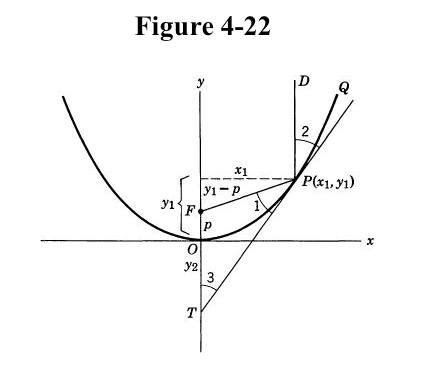
\includegraphics [scale=0.6] {Kline_4_22.png} \end{center}
Morris Kline has an alternate proof in his book \emph{Calculus}.  In the figure we need to show that angles $1$ and $2$ are equal.  By standard geometry angles $2$ and $3$ are equal, hence we need to show that angles $1$ and $3$ are equal.  We do this by showing that $FP$ is equal to $FT$.

Rather than substitute for $y = ax^2$ we just leave things in terms of $y$.  Notice that the diagram uses $p$ for the distance from the origin to the focus, and labels $P = (x_1,y_1)$.  Using Pythagoras, as indicated, the distance $FP$ is 
\[ FP = \sqrt{x_1^2 + (y_1-p)^2} \]

To get $FT$ we need to find what is labeled as $y_2$, the intercept of the tangent line with the $y$-axis.  We get this from the point-slope formula:
\[ \frac{y_1 + y_2}{x_1} = 2ax_1 \]
\[ y_1 + y_2 = 2ax_1^2 \]
But of course $y_1 = ax_1^2$ and so
\[ y_1 + y_2 = 2y_1 \]
Thus $y_1 = y_2$ and hence $FT = y_1 + p$.

Going back to $FP$, we use the same crucial fact about the focus that we relied on in the first proof, namely that $4ap = 1$ and so
\[ y_1 = ax_1^2 \]
\[ x_1^2 = 4p y_1 \]
Our previous expression was
\[ FP = \sqrt{x_1^2 + (y_1-p)^2} \]
substituting for $x_1^2$
\[ FP = \sqrt{4py_1 + (y_1-p)^2} \]
\[ = \sqrt{4py_1 + y_1^2 - 2y_1p +  p^2} \]
\[ = \sqrt{y_1^2 + 2y_1p +  p^2} \]
\[ = \sqrt{(y_1 + p)^2} \]
\[ FP = y_1 + p \]
$FT$ and $FP$ are the same length, and so the two angles are equal.  Also, we showed that $FP = y + p$, which means that every point on the parabola has the distance $y + p$ to the focus, as well as the vertical distance $y + p$ to a horizontal line a distance of $p$ below the $x$-axis and parallel to it.  This line is the directrix.


\end{document}